\chapter{SFC Implementation}
\label{chap:impl}

\newcommand{\enchainer}{\texttt{Enchainer}}
\newcommand{\vnf}{\texttt{VNF}}
\newcommand{\vnfs}{\texttt{VNFs}}
\newcommand{\dispatcher}{\texttt{Dispatcher}}
\newcommand{\astaire}{\texttt{Astaire}}
\newcommand{\ironhide}{\texttt{Ironhide}}
\newcommand{\harbor}{\texttt{Harbor}}
\newcommand{\roulette}{\texttt{Roulette}}
\newcommand{\ingress}{\texttt{ingress}}
\newcommand{\ingresses}{\texttt{ingresses}}
\newcommand{\egress}{\texttt{egress}}
\newcommand{\egresses}{\texttt{egresses}}

In this chapter there is described the implementation of the solution that we
proposed for the SFC system. Also the experimental implementation that allow us
to reach the final solution are discussed and why they where abandoned.

\section{Kubernetes Pods and our implementation}
\todo{Describing pods}

\section{How to reach virtual functions}
The first issue to overcome in our implementation was how to make possible to
reach Pods inside Kubernetes without specifying the IP of the machine on the top
of which they are running. In fact, enabling that possibility would allowed us
to create a flexible and scalable solution. In fact, decoupling Pods to physical
machine let our proposal to be independent on the underlying infrastructure: the
addition or the removal of hosts would be transparent for the code developed,
demanding to Kubernetes the task of manage the change in computational and
storage resources. Kubernetes services \todo{add reference} allowed us to
overcome the problem. \todo{add Kubernetes services explanation}

\subsection{Kubernetes Services}
A Kubernetes service is an abstraction that defines a set of Pods and policies
to access them. Pods referenced by a certain Service are usually selected with a
\emph{Label Selector}. In general these labels, added to Pod specifications,
does not provide uniqueness but identify a set of objects.
In the snipped~\ref{chap:impl:lst:srv} there is an example of Service
definition.The service create will be called \texttt{my-service} and targets TCP
port 9376 on any Pods labelled with the selector \texttt{app=MyApp}. Kubernetes
will assign to the Service an IP address (also called \emph{clusterIP}). 
\texttt{port} filed in the definition is the port on which the Service can be
reached, instead \texttt{targetPort} is the port on which traffic will be
redirected on Pods. It can be either a valid port number or a string that
identify port name of backend Pods, allowing more flexibility to Pod and Service
creation. Supported protocols are TCP, UDP and SCTP. \texttt{kube-proxy} is
accountable for implementing virtual IP for Services (other than Services with
type \texttt{ExternalName}). 

\begin{lstlisting}[caption={Example of Service definition},
                   captionpos=b, language=yaml, label=chap:impl:lst:srv]
kind: Service
apiVersion: v1
metadata:
  name: my-service
spec:
  selector:
    app: MyApp
  ports:
  - protocol: TCP
    port: 80
    targetPort: 9376
\end{lstlisting}

For Service discovery, there were \emph{environment variables} and \emph{DNS}.
To Pods running on a certain Node \texttt{kubelet} add a set of variables for
each Services, that can be used for referencing to it. In the former technique,
to discover services, instead, are used the DNS server cluster add-on. It
watches Kubernetes API to be aware if new Services are created to add DNS
records for them. In this way all Pods are able to do Service name resolution
automatically. Services types can be:
\begin{description}
\item[ClusterIP:] to expose services only within the cluster, it is the default
value;
\item[NodePort:] to expose the service on a static port. Outside the cluster is
reachable by requesting \verb!<NodeIP>:<NodePort>!
\item[LoadBalancer:] to expose a service externally, using a cloud provider
load balancer;
\item[ExternalName:] to expose a service with the name expressed in the 
\texttt{externalName}.
\end{description}

All services that we used belong to \texttt{NodePort} category. This choice was
made for a twofold reason. First is the sake of simplicity: binding services to
a predefined port is easy to concatenate services and identify them by port.
\texttt{NodePort} type is not suitable to expose services to the outside world,
as instead \texttt{ExternalName}. However it requires the registration of a
domain name. In a production ready platform or in a more advanced testbed,
alternative type of services can be used.

Taking advantage of that, we decided that all components of our solution that
will be deployed on Kubernetes will be exposed by a service. In this manner, to
reach a defined component in our solution it is possible to only specify the
name of the service and the port to which it is bound. Kubernetes is in charge
to decide which Pod to reach (if more replicas of the same function are
available) in the pool labelled to belong to the same service, resolving the
location on which it is deployed.

\section{First review}
\begin{figure}
  \centering
  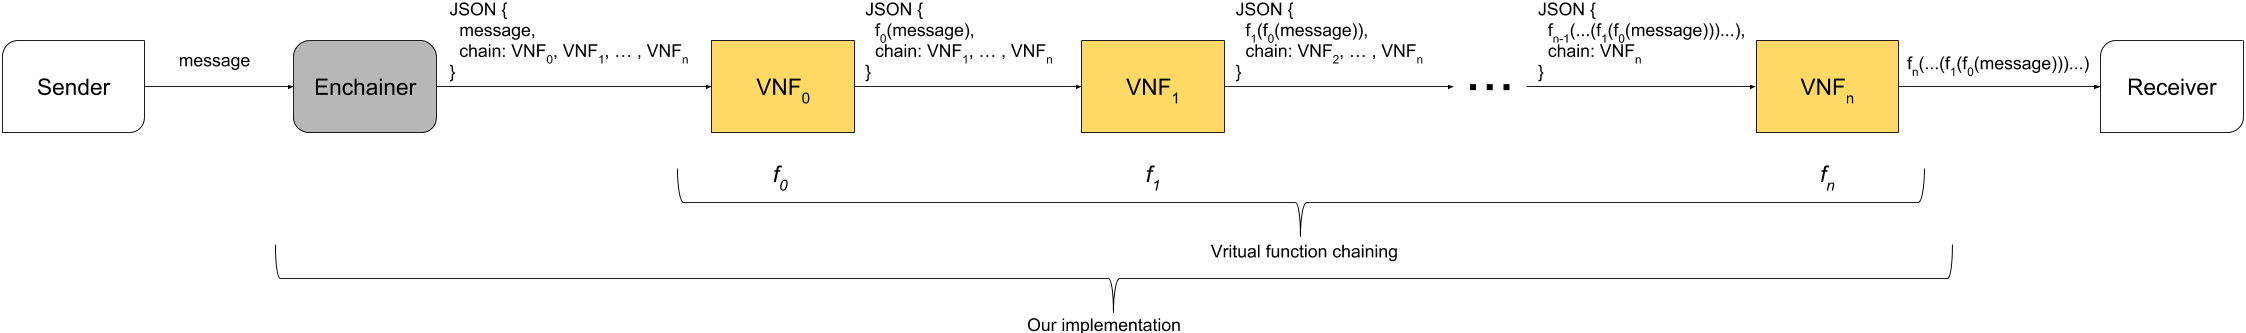
\includegraphics[width=\textwidth]{firstreview}
  \caption{First review schema}
  \label{chap:impl:img:firstreview}
\end{figure}
First SFC implementation was only developed to become familiar with
technologies, in particular with Kubernetes. At this stage of the project there
were not implemented yet any sort of automatic chain deployment. Moreover
there were not any mechanism to retrieve chain or function available and the
path that traffic must traverse were statically defined at the chain edge:
traffic inspection is not implemented and the classification is only simulated
returning always the identifier of the chain deployed. This first solution
schema is described in Figure~ \ref{chap:impl:img:firstreview}. Two components
were identified: \begin{itemize} \item \enchainer
  \item \vnfs
\end{itemize}
The former element represent the first link on each chain. The goal of this
element is to receive packets from the sender and, in a more evolved solution,
to query the classifier retrieving the SFC composition. After it wraps the
message into a JSON file, along with the path chain specification:
\begin{lstlisting}[language=json]
{
    "message" : "<the original message>",
    "chain": ["<IP vnf1>", "<IP vnf2>", ..., "destination"]
}
\end{lstlisting}
The \texttt{message} field is the original message sent to the chain,
instead the \texttt{chain} field is an array of IPs or Kubernetes service names
that allows to reach VNF. The array even specify VNFs order. The last element
must be the final destination of the packet. 
The \vnf{} in this review are seen as two layer application. One layer is
the ``real'' VNF, so the treatment of the traffic, the other, instead, manage
the communication in the chain. It must provide the capability to forward
packets following this schema:
\begin{enumerate}
  \item once a packet arrives the field \texttt{message} must be read and the
  function represented by the VNF applied;
  \item the field \texttt{chain} must be read and based its values there are two
  possibilities:
  \begin{enumerate}
    \item if array length is greater then $1$ the JSON that wraps the message
    must be reconstructed because the actual \vnf is not the last
    element of the chain. \texttt{message} field must be set to the result of
    of the function application and the \texttt{chain} field must be updated
    removing the first element of the array;
    \item if array length is equal to $1$, after the application of the
    transformation of the VNF to the value of the \texttt{message} field,
    message must be delivered to destination, without the JSON wrapping:
    \item in other case message must be discarded.
  \end{enumerate}
\end{enumerate}

\subsection{Implementation}
This first code implementation was developed in Java\footnote{And available on
this repository: \\\url{https://github.com/Augugrumi/chaining-functionalities}}
The \enchainer{} component is simply a server implemented using Netty
library\footnote{\url{https://netty.io/}}. The choice of this framework is due
the possibility to serve multiple protocols and for its quick and easy usage. 
The \vnf{} component is defined as follow: an interface define methods
that must be implemented, an abstract class extends the previous interface
implementing the communication layer of the interface as well as it manages the
JSON wrapping/unwrapping. \vnf{} communication take advantage of
Rapidoid\footnote{\url{https://www.rapidoid.org/}} library for packet sending
and receiving, both for simplicity and because it gives the opportunity of
managing a large pool of connection in a rapid way. In this prototype solution
it is possible to replace the \vnf{} component with every element that
provides the same JSON wrapping management logic and that gives is capable
to send and receive packets. Java code could be implemented with the different
VNF but alternative implementations (even developed in different languages) are
allowed. 

\subsection{Kubernetes Deployment}
Two alternative approaches where implemented to deploy chain exploiting this
solution: using a single Pod or multiple Pods. First solution, although easier
to deploy is not scalable: all the components of the SFC will run on the same
Kubernetes Node. Second approach make use of different Pods.

\subsubsection*{Single Pod}
To deploy the first review solution using a single Pod the SFC composition is
defined using a single Kubernetes Deployment (in which all the \vnf{} and
the \enchainer{} are specified) and a single Service that exposes the
\enchainer{} and makes it reachable outside the Pod using the Service name.

\subsubsection*{Multiple Pods}
Multiple Pods first review follow a different approach. For each \vnf{}
and for the \enchainer{} is defined a different Deployment and a Service.
Even if it is more cumbersome to define chain like this it helps to create a
more scalable and flexible solution. In fact, exposing each \vnf{} with a
Service allows the single \vnf{} to be part of different SFC and to do not
have static chain created at deployment time. Moreover, handling separately
the components make possible to increase/decrease the number of single
\vnfs{} or of the \enchainer{} basing on traffic load.

\subsection{Problems}
This first attempt has different issues. First \enchainer{} has no
possibility to retrieve all the original message of a sender: it requires at
least that even the transport layer headers can be read, but it is not possible
due to i) server created with Netty works at application layers and ii) Java
does not allow to create socket at an enough low layer that allow transport
layer header reading. To mitigate this and deploy the solution the workaround
was to add to the payload of the message sent the missing headers. Lower layer
header allows the classifier (that is not implemented) to know more information
on the communication, so to perform a better analysis on the treatment to apply
on the incoming packets. Another problem was the JSON wrapping: it does not
follow the standard encapsulation defined for this technology. Passing to a
standard encapsulation was planned, but the JSON one was useful because of the
format, that can be easy read and write. Further, even the communication among
VNF works at application level using POST request to sends data and lower layer
communication can enhance performance. Finally, with this implementation data
sent from the sender must be fully received to the \enchainer{} before, then
from each \vnf{} in the chain, making communication slower and making it not
suitable in some context such as transfer of heavy files.

\section{Second review}
\begin{figure}
  \centering
  \includegraphics[scale=0.2]{secondreview}
  \caption{Second review schema}
  \label{chap:impl:img:secondreview}
\end{figure}
The second review is an enhancing of the first proposal in which components
organization is changed, as depicted in Figure~\ref{chap:impl:img:secondreview}.
Main goal of this review were to further study technologies involved into the
project and to examine a different approach.

Simultaneously of the development of this proposal we started the development of
the instrumentation that automatize the chain deployment.

In this second proposal three components are defined:
\begin{itemize}
  \item \enchainer{}
  \item \dispatcher{}
  \item \vnfs{}
\end{itemize}
\enchainer{} is pretty the same of the first implementation. Even in this case
the this component must be the first element to be traversed of the chain, that
wrap the message into a JSON format as in the previous solution and define the
list of function that traffic must traverse. \vnfs{}, instead, were revisited.
During the development of this second implementation we thought that they must
be decoupled to the mechanism on encapsulation, leaving to \vnf{} only the task
to perform the function to transform traffic and to implement basic
communication functionalities, as receive a packet and give back a response. The
new element introduced was the \dispatcher{}. It was a centralized component
whose aim is to manage the chain composition and work in this manner: it receive
the JSON wrapped message from the \enchainer{} and retrieve both
\texttt{message} and \texttt{chain} fields values. After it sends the former
value to the first element of the array described from the \texttt{chain} field.
Following this idea, \vnfs{} does not need to know anything about the JSON
formatting (\emph{SFC unaware}) but it only to be able to receive packet on a
certain port, (eventually) modify it and send it back. Basically, the different
approach compared to the previous implementation depends on the presence of the
dispatcher that is accountable of the traffic forwarding.

\subsection{Implementation}
Even this second implementation experiment was developed in Java\footnote{And
available on this repository: \\
\url{https://github.com/Augugrumi/alternative-chaining-functionalities}}. The
\enchainer{} implementation basically was not changed. To the \vnf{} component
was removed the JSON encapsulation code: as in the previous review a hierarchy
is provided, but this time is only need for a more rapid function development.
Even this prototype allow to create \vnf{} using different code or programming
languages, only requirements are:
\begin{itemize}
  \item to be able to receive a POST request;
  \item to be able to modify the payload of the POST request, applying the
  function for which it was created;
  \item to be able to reply to the previous request, sending the modified data.
\end{itemize}
The code managing wrapping is moved to the \dispatcher{}, that make use of
Rapidoid library for ingoing and outgoing communications.

\subsection{Kubernetes Deployment}
Even for this implementation we provide two different deployments, one that
deploy all the system in a single Pod and the other that exploit the possibility
to use multiple Pods. The deployments works as before. In the Single Pod one the
SFC, the \enchainer{} and the \dispatcher{} are specified onto the same
Deployments and a Service is specified to be able to reach the chain. In the
Multiple Pods deployment, as before, each component is defined by a different
Deployment and exposed by a Service.

\subsection{Problems}
This second review, since it is based on the code of the previous one, does not
solve the problems explained before, as the problem regarding application
level communications, the usage of Java as programming language and JSON
wrapping issues. This solution was developed to study a different topology
approach, using a centralize element, the \dispatcher{}, that can be the traffic
orchestrator and can redirect traffic to the \vnfs{}. Also, improving its
capabilities, it could have more information on transformation that packets must
pass through and eventually, reclassify the traffic querying the classifier.
Moreover it provides a total decoupling between SFC platform and network
function that must be applied. Thus, there is the drawback of the centralized
approach. This limit the overall scalability since all function must talk to the
same component. Exploiting Kubernetes functionalities it is possible to augment
replicas of the \dispatcher{}, even automatically. Nevertheless, this approach
seems to be not suitable for large traffic loads and it could be the bottleneck
of the platform.

\section{Final proposal}
After the second review we performed a complete change in terms of
implementation and technologies used. We redesigned the possible solution based
on the problems that we found on the first and the second reviews. The final
proposal is composed mainly by $4$ components:
\begin{itemize}
  \item \astaire{}
  \item \harbor{}
  \item \ironhide{}
  \item \roulette{}
\end{itemize}
All together they provide the possibility to both create a chain of VNF and
handle it, allowing the automatic deployment.

\subsection{Classification}
One of the killing feature of the SFC platform is the capability to classify
traffic based on its typology. In fact, this make the system able to redirect
traffic load on the more appropriate chain of network function and, if needed,
to change the treatment during SFC traverse. Nevertheless, even in the final
implementation we does not take into account the development of a fully featured
classifier because it is outer of the scope of this project, although the
latter element is considered in the overall system functioning but is
implemented only as a mock component: based on the protocol type used on
transport layer used to transmit traffic to the SFC edge, it gives back a
chain identifier. The protocol supported are only TCP and UDP.

\subsection{Packet transmission strategies}
When packets are sent from a sender $S$, to a receiver $R$, in this scenario,
they start travelling to the network and reach the our system, where traffic can
be classified and redirect to the appropriate SFC to be handled. During this
elaboration, it is important to maintain transparency (making the sender unaware
of what is happening in the middle of the transmission) and to keep all the
information of the original packet (headers included) for better classification.
To achieve this two main possibilities can be used TUN/TAP tunneling or
encapsulation packets such as IP in IP or TCP over TCP.

\subsubsection*{TUN/TAP}
\begin{figure}
  \centering 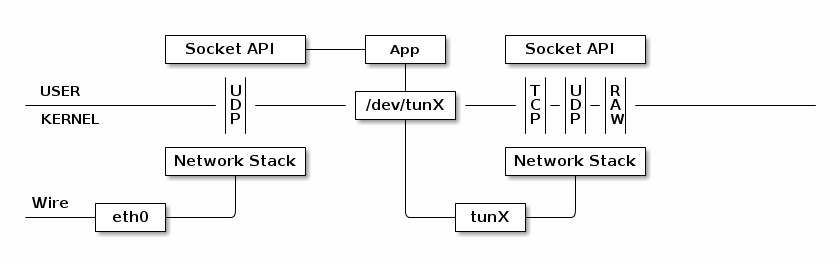
\includegraphics[scale=0.5]{tuninterface}
  \caption{TUN interface representation}
  \label{chap:prjan:img:tun}
\end{figure}
TUN and TAP are virtual kernel interfaces that do not have any physical
component differently to usual network interfaces. TUN (network TUNnel) operates
at level 3, as IP packets, TAP (network tap) instead at layer 2, dealing with
Ethernet packets. Using them in user-space programs they emulates the incoming
of data from external sources injecting packets to the operating system stack.
Interfaces can be created as transient (created and destroyed from the same
program) or persistent (created by some utility and programs attach to them) and
once created they are seen as hardware interfaces. In network tunnels created
using this interfaces it is possible to exchange data in secure way over a
public network as to transmit packets trough a network even if a certain protocol
is not supported, thanks to the encapsulation. This encapsulation allow, thus,
to maintain unaltered packets inside the tunnel.

\subsubsection*{Packet encapsulation}
\begin{figure}[t]
  \centering \includegraphics[scale=0.5]{IPoverIP}
  \caption[IP Encapsulation within IP packet schema]{A schema of IP
    Encapsulation within IP. Is noticeable how the original packet becomes the
    payload of a new one, thus being encapsulated. All the information
    regarding the original packet remains untouched: when this kind of packet
    gets send from a machine to another, the OS will remove the new packet
    header and will present to the user-space program receiving the data its
    payload: a IP packet. Packets encapsulation can be applied with higher
    layers too, thus allowing for TCP and UDP packet encapsulation.}
  \label{chap:prjan:img:ip_over_ip}
\end{figure}
IP in IP encapsulation allow to preserve the original packet making it to
become the payload of a new packet, that can be elaborated and modified
accordingly, until it gets decapsulated and sent to the receiver eventually.
When it receives the packet, it is not be aware of the packet elaboration, since
all the original headers were preserved (or slightly modified). In particular,
IP in IP allow the packets to pass through intermediate destinations that
otherwise would not be selected. Split-TCP, instead, ``divide'' the TCP session
in two parts using proxies: each proxy pretends to be the opposite endpoint in
each direction. It creates a multi-overlay-hop path where for each hop there is
an possible independent TCP connection. In order to achieve that, a session
table needs to be established and continuously updated, while TCP headers need
to be accordingly modified to allow data transmission through the proxies and
endpoints. Nonetheless, care should be given to packets path: in order to avoid
ill-calculated congestion windows, the incoming packets need to follow the same 
(or an equivalent one) path for the same instantiated connection. This
phenomenon is based on the intermediate proxies that create the route: it is the
case, for example, when an intermediate node sends back a spoofed ACK before the
original packet is delivered to the real consignee. In this scenario, the
sender, unaware of the proxy, will miscalculate the sending window based on the
too low RTT. Other problems of TCP splitting are reliability and security,
especially because the end to end TCP logic is no longer maintained: a server
failure may cause to an unaware client to believe that all the packets have
reached the destination. TCP session recreation seems burdensome and it doesn't
seem to add any significant benefit at the first sight, but it offers the
flexibility to perform extensive packet manipulation and use different TCP
flavors hence increasing performance in heterogeneous networks.

\vspace*{1cm}

\noindent In the final review we tried both the two approaches. The tunnelling
approach is not suitable for communication among different links of the chain:
in fact it will create a strong relation among the Pods, nullifying the use of
Kubernetes services. Moreover, Pods are mortal and if a Pod die in the tunnel,
time is required to reconstruct it. Finally creating a tunnel make more
difficult to update a chain or reclassify a packet during the SFC traverse
because different tunnel must be created. Also, using a TUN tunnel the
communication between the external world and the SFC would be more cumbersome.
At the other end it will make possible to keep all the headers of the original
packets easily and make more secure the communication. Encapsulating packets
give us a more flexible approach and we decided to utilize it even if it does
not allow us to keep header information in a simple manner. Both for TCP and for
UDP external connection, the communication among links in the chain uses UDP
protocol: it is an unreliable protocol but it is lightweight and allow a faster
packet transmission compared to TCP.

\subsection{Ingresses end egresses}
In both of the previous implementation there was a component that handle the
traffic before it traverse the chain. In this final solution we developed 
\ironhide{}\footnote{\url{https://github.com/Augugrumi/ironhide}}. This
component is useful not only to manage incoming packets but even the
communication with the final destination. We called the element of the solution
that is accountable for the treatment of incoming packets \emph{ingress} and
similarly the component that handle the communication with the destination is
called \emph{egress}. \ironhide{} is developed in C++ provide all the
functionalities to handle incoming packets from the outside of the chain and to
deliver packet after the SFC treatment. When \ironhide{} works as ingress it
basically operates as a server that accepts both TCP and UDP packets. Once a
packet arrives it is forwarded to the classifier, along with the TCP/UDP-IP
headers, make decision on the SFC to which it must be forwarded.

The result of the classification is used in the creation of the NSH. During the
implementation of our solution we only considered the SFC encapsulation with
Fixed-Length Context Header: we reduce as possible the usage of metadata to be
exchanged within the header to be as independent as possible to the header
typology, and the semantic is represented in Figure~\ref{chap:impl:img:nsh}.

\begin{figure}
  \centering 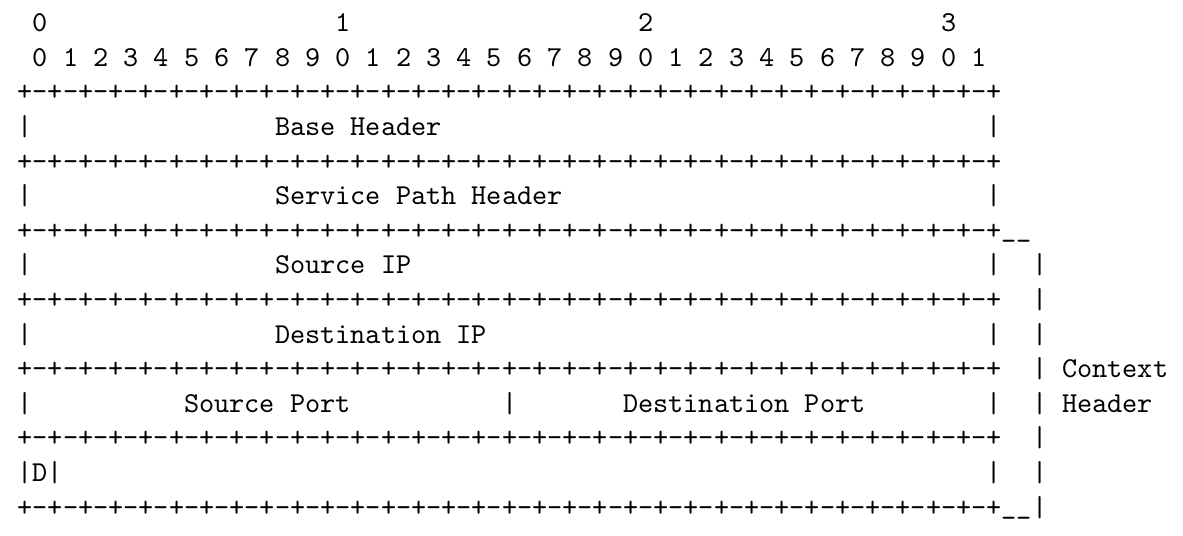
\includegraphics[scale=0.5]{nshsol}
  \caption{NSH Fixed-Length Context Header field usage}
  \label{chap:impl:img:nsh}
\end{figure}

The \texttt{Base Header} part of the header is used as defined in the RFC 8300.
The \texttt{Service Path Header} has a little difference. In fact the 
\texttt{Service Path Identifier} is used as described into the standard but the
usage of \texttt{Service Index} slightly differ. The RFC defines that in must
start with all bits set to 1 an each time the packet pass through a link the
field value have to be decremented. We has done the opposite only for the sake
of clarity and simplicity. A further improvement of the code could only compute
the opposite of this field. The \texttt{Context Header} is decomposed in:
\begin{description}
  \item[Source IP:] 32-bit representation of IPv4 original source address;
  \item[Destination IP:] 32-bit representation of IPv4 original destination
  address;
  \item[Source Port:] 16-bit representation of port used by the packet source;
  \item[Destination Port:] 16-bit representation of port used by the destination
  to receive packet;
  \item[Direction (D):] 1-bit chain traversal direction representation.
\end{description}
The first 4 fields are necessary to make the solution independent to carry along
the chain information about endpoints. IPv4 representation is used but
improvements and use of variable length context header can enhance the
solution allowing both IPv4 and IPv6 address representation. The 
\texttt{Direction} bit instead is used to make components of the chain aware of
the direction on which the SFC is traversed. This field is not strictly
necessary but allow to retrieve this information without retrieving it checking
actually which is the previous link that has managed a given packet. 

Finally, before delivering the packet to the first element of the chain the
\ingress{} record an entry on a local map to remember the connection with
the sender of the message. It of paramount important in bidirectional
communications: in fact the connection with the sender is kept alive to
subsequently deliver the answer of the receiver. In fact, if the latter sends
back data to the sender, the \ingress{} is able to deliver it thanks this
information saved.

\texttt{Egress} component wait for communication from the chain an it is in
charge to forward messages to the destination initially specified from the
sender before the manipulation of the SFC. To accomplish this task is
accountable to establish a connection, TCP or UDP depending on the original
sender communication parameters, with the final receiver. Delivering the final
packet it establish a connection and, as in the \ingress{}, this information is
saved into a map. 

\subsection{Roulette}
In bidirectional communication, that involves a continuous interaction between a
sender and a receiver, it is needed to not only keep the connection alive
between sender/receiver and \ingress{}/\egress{} but even to make possible to
retrieve the \ingress{}/\egress{} in case of a set of replicas of these
components are deployed.

\begin{exmp}
Suppose we have a set $I=\{I0, I1, I2\}$ of \ingresses{} and a set $E=\{E0,
E1\}$ of \egresses{} and suppose that from the sender $S$ packets reach the
destination $R$ following the path:
\begin{verbatim}
S -> I0 -> sfc -> E1 -> R
\end{verbatim}
If the response does not reach again the ingress $I0$ but $I2$, the connection
between $S$ and $I0$ must be aborted and a new connection among $S$ and $I2$
must be established. The same is whether different \egresses{} are used. This
semantics requires modification both on sender and on receiver at the
contrary of using always the same \ingress{} and \egress{} for a given
connection.
\end{exmp}

To accomplish this goal we developed \roulette{}. This component orchestrate SFC
ingresses and egresses in this way: once a new connection is open on a certain 
\texttt{ingress}, the latter has the task to save on \roulette{} database an
entry specifying its information (IP), on the communication and on the SFC used.
Once the packet has traversed the whole chain and reach an \texttt{egress} the
same entry is updated, adding even the \texttt{egress} information. Thanks to
this component it is possible to bind a communication to a specified pair 
\verb!<ingress,egress>!.

\roulette{}\footnote{\url{https://github.com/Augugrumi/roulette}} was developed
in Java using Spark\footnote{\url{http://sparkjava.com/}} to manage requests and
connected to a MongoDB\footnote{\url{https://www.mongodb.com/}} database. We
choose MongoDB as database because it allows to have a flexible data schema,
useful in particular in a test environment.

\roulette{} sake is not only to manage \ingresses{} and \egresses{} information
but it also keep the definition of the chains. in fact once a classifier return
the identifier of the SFC that traffic must traverse, the complete definition
or the link of the chain in a certain position can be retrieved querying this
component. SFC definition follow this pattern:

\begin{lstlisting}[caption={Definition of an SFC}, captionpos=b, language=json]
{
  "si" : [
    {
      "url" : <vnf0-service-name>,
      "port": <vnf0-port>
    },
    ...,
    {
      "url" : <vnfn-service-name>,
      "port": <vnfn-port>
    }
  ]
}
\end{lstlisting}

where the \texttt{si} field is an array of objects that identifies a single VNF
that belong to the chain. it is composed by the field \texttt{url} in which the
identifier of the service that allow to reach a certain VNF is specified and the
field \texttt{port} specify the port that must be used to contact the service.

We choose to use the same component for both SFC definitions and 
\ingress{}/\egresses{} pairing only for time constraint. There are not other
limitation that impose that these two pieces of information must be handled by
the same component. 

As the chains, \roulette{} is deployed on Kubernetes using a Service to expose
its functionalities. Use of Kubernetes allows even to have a database replica to
avoid data loss and high availability of information.

\subsection{Proxies}
\texttt{Ingresses} are implemented as a server that allows both TCP and UDP
connection on a given port. In order to do so are used \verb!SOCK_STREAM! and
\verb!SOCK_DGRAM! socket respectively. This approach has a drawback: opening
this kind of sockets does not allow to read even the TCP/UDP-IP headers of the
incoming packets. In a mirrored way, \egresses{} open same type of sockets to
communicate with the destination, so neither in this case it is possible to read
headers. To preserve them we implemented a workaround in form of a Python script
that recreate original header that must be put between the sender/receiver and
the \ingress{}/\egresses{}, that works as a proxy that add to the payload of the
original message even the header recreated. This script was developed both for
UDP and TCP protocols.

The solution can be enhanced removing the proxies exploiting
\texttt{raw sockets}. Redesigning \ironhide{} to make it able to manage level 2
communication (Ethernet packets) will make that every packet received will
be read along with its headers. This approach has a main disadvantage: in TCP
connections part of the TCP logic must be re-implemented, as TCP-IP header
creation or ACK handling. For this reason we does not implemented it. UDP
instead does not requires too much modification and communication between 
\egress{} and the destination was developed using level 2 sockets: this even
shows that proxies are not necessary components of the solution proposed but
they are only needed due to our implementation.

\subsection{Astaire}
The component that enable the communication with VNF and the creation of chains
is \astaire{}\footnote{\url{https://github.com/Augugrumi/Astaire}}. This
component, developed in C++, implement the SFF in the traditional architecture
overview. As mentioned before, communications among \ingresses{}/\egresses{}
and VNFs and among virtual functions each other are implemented using UDP
protocol. This choice was made due to the fact that UDP is lightweight and in
general faster than TCP, event thanks to the smaller header. 

\astaire{} main tasks are to receive and forward packets and it is implemented
as a SFF that manage a unique VNF. Since we suppose that all the VNF that our
system manage are SFC unaware we incorporated the NSH handling and SFC proxy
functionality in this element. To deal with SFC aware only modification required
is to not remove this encapsulation. Basically once a packet is received it
remove the NSH encapsulation and send it to the associated virtual function. In
this implementation we suppose that \astaire{} is able to reach a VNF as a
simple method call or invoking a C++ or Java program whose path is passed to 
\astaire{} as argument during launch. The VNF must be able to manage an array of
bytes that represent the packet that is traversing the chain, to which is
removed the NSH (so headers and payload of the original packet, eventually
modified from previous virtual functions). Call to VNF is totally decoupled
to forwarding mechanism, so it could be expanded allowing the possibility to
call a function in terms of sending a packet and waiting for the response. When
the VNF has finished to treat the packet, based on the NSH removed before,
calculate the next step of to which forward traffic and the new header. 

To retrieve the next element \astaire{} reads the \texttt{Service Path
Identifier} and the \texttt{Service Index} fields of the \texttt{Service Path
Header}. After it checks in a local map if this values was used yet: in this
case in the map are saved information (address, port) of the next element.
Whether this information is not present it have to query \roulette{} to recover
this data. The \texttt{Service Index} field is incremented before this check. In
case the instance of \astaire{} is the last link of the SFC roulette will
return:
\begin{itemize}
  \item the name of the \egress{} service in case that the current packet is the
  first packet that traverse the chain exchanged between a certain pair
  $<sender,receiver>$; or
  \item data of the \egress{} used for the actual communication.
\end{itemize}
Local maps update its information periodically in an automated way: this make
possible to be responsive to SFC updates or changes on Pods configuration. The
update period is set to 2 minutes by default but further enhancement must set it
more accurately. Since Pods are mortal for their nature a system to detect fault
and update local maps: this will make the overall platform less prone to packet
loss.

The new NSH that \astaire{} will add to the packet to send will have the field
\texttt{Time To Live} decremented by one and the field \texttt{Service Path
Identifier} increased by one. This mechanism also prevent the creation of
cycles: as a metter of fact that either the \texttt{TTl} field will goes to $0$
and the packet will be discarded or the \texttt{SPI} will no more point to an
element of the chain and traffic will be redirected to an \egress{}.

\subsection{Chain management}
To handle chains and virtual functions we developed
\harbor{}\footnote{\url{https://github.com/Augugrumi/harbor/}}. This component
work as the MANO of our platform. We developed \harbor{} in a manner that it
is not possible to deploy single VNFs. This because the single VNF does not
allow the management of incoming and outgoing traffic without \ingresses{} and
\egresses{}. This component is only a prototype of a fully featured orchestrator
even regarding VIM handling. In fact, due to time contraint the communication
with Kubernetes APIs is implemented only on a basic level, allowing only some
operation. It is implemented in Java using Spark to expose a REST API with which
is possible to handle SFCs. Despite other components of this implementation 
\harbor{} is not deployed on Kubernetes.

\harbor{} handle both VNF and SFC catalogs: it is possible to get the list of
saved definitions, to add and update an existing one and to remove one of them.
Moreover, since it is an orchestrator it allows to launch a new SFC instance
from a previous saved definition and to stop a running chain instance.

An example of VNFs and SFC that can be deployed using \harbor{} and our platform
is showed below. In~\ref{chap:impl:lst:vnfexample}. As explained in \todo{add
reference to service} all the function that will run on Kubernetes are exposed
using a Service, decoupling the use of a certain function to the way it can be
called.
\begin{lstlisting}[caption={Example of VNF definition}, captionpos=b,
                   language=yaml, label=chap:impl:lst:vnfexample]
kind: Deployment
apiVersion: extensions/v1beta1
metadata:
 name: astaire-deployment
 namespace: default
 labels:
   k8s-app: astaire-vnf
spec:
 replicas: 1
 selector:
   matchLabels:
     k8s-app: astaire-vnf
 template:
   metadata:
     labels:
       k8s-app: astaire-vnf
       name: astaire-vnf
   spec:
     containers:
       - name: astaire
         image: augugrumi/astaire:latest
         args: ["-u", "-r", "roulette-service:80"]
         imagePullPolicy: Always
         ports:
           - name: udp
             containerPort: 8767
             protocol: UDP
---
kind: Service
apiVersion: v1
metadata:
 name: astaire-service
 namespace: default
spec:
 selector:
   k8s-app: astaire-vnf
 ports:
   - name: udp
     port: 8767
     protocol: UDP
 type: NodePort
\end{lstlisting}

In~\ref{chap:impl:lst:sfcexample} is shown an example of SFC definition. It is
implemented using only as an array of VNFs definition. The array gives even the
order of the functions in the chain.
\begin{lstlisting}[caption={Example of SFC definition}, captionpos=b,
                   language=json, label=chap:impl:lst:sfcexample]
{
    "ns" : [
                {
                    "id": "astaire-service"
                },
                ...
            ]
}
\end{lstlisting}

Once a definition of a chain is updated, this transformation is reflected to
running intances of the SFC (if any) to make the system more flexibile.
Monitoring functionalities implemented are really limited: \harbor{} can only
provide information if a certain SFC is running and if components of that SFC
instance are running. At this stage it is not developed to provide data on Pods
faults or misbehaviours. Furthermore, not scalability features are implemented
yet.

Finally, this architectural component has the task to set the description of
running chains on \roulette{}.

Since \harbor{} is the MANO has to instantiate the SFCs routes that 
\ingresses{}, \egresses{} and \astaire{} instances can use. 

\section{Implementation problems}
This final solution has still some issues both due to how we implemented the
whole system and time constraints. \harbor{} is only an experimental
implementation: as stated before a fully fuctional MANO must be able to provide
more information on running SFCs and VNFs. In addition, the possibility to
manual scaling element of a running chain can improve even more this component.
Definition of the VNFs allows to define the ReplicaSet (since they are YAML
file used by Kubernete) but a future release of this component must provide
the possibility to define roules to autoscale. Kubernetes enable this
opportunity taking advantage of \texttt{autoscaling/v2beta2} API
version\footnote{\sloppy\url{https://kubernetes.io/docs/tasks/run-application/horizontal-pod-autoscale-walkthrough}},
in which the set of Pods can be increased/decreased basing on specified metrics.

\roulette{}, that has to keep track of chain endpoints (the pair $<\ingress{},
\egress{}>$) of a communication and the SFCs instances deployed, is a
centralized element of the platform, as it is used and implemented in this final
review. It was thought as element on which the blocks of the final proposal have
to most frequently perform reads than writes, but increasing the number of
connection that exploit the chain this implementation can be not enough and a
distributed and more scalable approach have to be used. An alternative solution
is to divide it into two different element: one that gives to endpoints and to 
\astaire{} instances information on the chain and one that take care of pairing
ingresses and egresses. The former components will be written only by the MANO.
The latter piece of information can, instead, be added to a variable length NSH.
Exploiting this possibility the platform will have a lighter backend and the
pair $<\ingress{}, \egresses{}>$ will be added directly from this components to
the header and forwarded by \astaire{}. 

\texttt{Ingresses} and \egresses{} implementation problems lay on the socket
handling. Low level socket must be used in a future implementation, making
endpoint able to read headers and to be performance enhancement proxies. Another
improvement is to better support end-to-end communication between sender and
receiver. If sender (or the receiver) disconnects from the corrispondant
endpoint it is transparent to the counterpart. The same happens in case of
packet loss. Mechainism to manage these scenarios must be develop (as, in
general, proxies are used).

The communication inside the patform take advantage of the lightweight UDP
protocol approach but does not internal mechanisms of packet recovery. It could
be useful to implement some sort of local retransmission in case of packet loss
to avoid to give this responsability to the external sources.

Finally, \astaire{} is implemented as an SFF that take care of only one VNF. It
descrease complexity of component but it implies that one \astaire{} instance
must run for each VNF instance. Moreover our solution is only a simple
implementation and we do not tested it under a large traffic load, where right
connection handling has a critical role.

